\section{Results and Discussion}

\subsection{Problem 1: Cholesky Factorization and Linear System}

The prescribed matrix $A \in \mathbb{R}^{10 \times 10}$ is symmetric by construction. Furthermore, it is strictly positive definite. The algorithmic assembly defines $A = B B^T + 10 I$. For any non-zero vector $x \in \mathbb{R}^{10}$, the quadratic form is bounded strictly away from zero:
\begin{equation}
    x^T A x = x^T (B B^T + 10 I) x = \|B^T x\|_2^2 + 10 \|x\|_2^2 > 0.
\end{equation}
Consequently, $A$ is symmetric positive definite (SPD), guaranteeing the existence and uniqueness of the Cholesky factorization $A = G G^T$.

The numerical computation of the lower triangular Cholesky factor $G$ yields:
\begin{equation}
    \resizebox{0.95\textwidth}{!}{%
        $G = \begin{pmatrix}
                10.9545 & 0       & 0       & 0       & 0       & 0       & 0       & 0       & 0      & 0      \\
                0.5477  & 11.0770 & 0       & 0       & 0       & 0       & 0       & 0       & 0      & 0      \\
                2.1909  & -2.5458 & 8.4687  & 0       & 0       & 0       & 0       & 0       & 0      & 0      \\
                -5.6598 & 4.7937  & 4.6765  & 6.7169  & 0       & 0       & 0       & 0       & 0      & 0      \\
                -1.2780 & -7.6104 & -1.0125 & -1.9379 & 6.9763  & 0       & 0       & 0       & 0      & 0      \\
                3.0125  & -1.1420 & -4.7832 & -0.9092 & -1.3540 & 6.4095  & 0       & 0       & 0      & 0      \\
                -6.2988 & -0.5010 & 3.0140  & -0.1999 & -5.6189 & 0.3166  & 8.2023  & 0       & 0      & 0      \\
                -2.3735 & 1.9229  & -5.0663 & -1.6315 & -2.2491 & 1.3393  & -1.3539 & 9.0363  & 0      & 0      \\
                0.8216  & 2.0357  & 2.7611  & -0.3009 & 1.3984  & 0.7296  & -1.8971 & 2.8919  & 7.3496 & 0      \\
                -2.5560 & -3.4847 & -3.3383 & -1.3623 & -0.6890 & -1.7815 & 3.1255  & -0.9333 & 0.5297 & 5.7231 \\
            \end{pmatrix}$%
    }
\end{equation}
To verify the factorization, the reconstruction residual was calculated as $\|A - G G^T\|_2 \approx 1.096 \times 10^{-14}$, confirming numerical exactness near machine precision.

The $2$-norm condition number of the matrix was computed as $\kappa_2(A) \approx 29.23$.
Using the factor $G$, the linear system $Ax = b$ was solved via forward and backward substitution. The computed solution vector is:
\begin{equation}
    \resizebox{0.95\textwidth}{!}{%
        $x = \begin{pmatrix} -0.3351 & 0.1371 & -0.2335 & -0.7980 & -0.1570 & -0.5325 & 0.2272 & -0.0749 & 0.2875 & -0.2869 \end{pmatrix}^T.$%
    }
\end{equation}
The algebraic accuracy of this solution is verified by the residual norm $\|Ax - b\|_2 \approx 2.1168 \times 10^{-14}$.

\subsection{Problem 2: Original Finite-Difference Formulation}

The original discrete problem was executed exactly as prescribed by Code 2 using the seed $31837$. This generated the parameters $k = 0.2567$, $f = 1.9530$, grid spacing $h=0.1$, and selected the Neumann--Dirichlet boundary condition corresponding to $T'(0) = 0$ and $T(1) = 0$.

The resulting linear system $M_{orig} T_{orig} = s_{orig}$ was solved computationally. The numerical residual is $\|M_{orig} T_{orig} - s_{orig}\|_2 \approx 1.8253 \times 10^{-15}$. This negligible residual verifies that the linear system was solved correctly from a strictly algebraic perspective. However, a scientific analysis requires assessing the consistency of this generated system with the continuous model stated in the assignment.

The assignment mathematically defines the steady-state heat equation as:
\begin{equation}
    -k T''(x) = f, \quad x \in (0, 1).
\end{equation}
Subject to the Neumann--Dirichlet boundary conditions, the exact analytical solution can be derived by integrating the constant source term twice:
\begin{equation} \label{eq:exact-solution}
    T_{exact}(x) = \frac{f}{2k} (1 - x^2).
\end{equation}
Given $k, f > 0$, the analytical solution has specific qualitative properties: it is non-negative on $[0,1]$, strictly concave downward ($T''(x) = -f/k < 0$), reaches a global maximum at the insulated boundary $x=0$ ($T_{exact}(0) \approx 3.8039$), and monotonically decreases to the fixed temperature at $x=1$.

A rigorous diagnosis reveals that the prescribed discrete formulation is not consistent with the continuous differential equation stated in the assignment. Specifically:
\begin{enumerate}
    \item \textbf{Sign inconsistency:} The interior matrix coefficients $(1/h^2, -2/h^2, 1/h^2)$ approximate the positive second derivative $T''_{i}$, omitting the required negative sign in the Laplacian operator.
    \item \textbf{Source scaling inconsistency:} The generated right-hand side is $s_i = (h^2/k) f$, which improperly scales the source by $h^2$. Together with the sign inconsistency, the interior nodes inadvertently model the equation $T'' = \frac{h^2}{k}f$.
    \item \textbf{Boundary condition inconsistency:} The first row implements $\frac{1}{h^2}(T_1 - T_0) = \frac{h^2}{k}f$. Instead of imposing $T'(0) = 0$, this creates a mesh-dependent Neumann condition proportional to $h^3$.
\end{enumerate}
Consequently, at the prescribed grid resolution $h=0.1$, the original formulation produces a qualitatively different temperature profile. As shown in \autoref{tab:temperature-comparison}, its maximum absolute error relative to the analytical solution of the stated continuous problem is approximately $3.8457$. This discrepancy is attributable to the inconsistency of the discrete equations with the stated continuous model, rather than to failure of the linear solver.

\subsection{Problem 2: Corrected Formulation}

To construct a finite-difference system mathematically consistent with $-k T'' = f$, a corrected formulation was implemented. For the interior nodes ($1 \le i \le 9$), the standard central difference approximation was used:
\begin{equation}
    -\frac{1}{h^2} T_{i-1} + \frac{2}{h^2} T_{i} - \frac{1}{h^2} T_{i+1} = \frac{f}{k}.
\end{equation}
For the Neumann boundary at $x=0$, a first-order forward difference approximation was applied to impose $T'(0) = 0$:
\begin{equation}
    -\frac{1}{h} T_0 + \frac{1}{h} T_1 = 0.
\end{equation}
The Dirichlet boundary at $x=1$ is strictly enforced via $T_{10} = 0$. This corrected linear system, denoted $M_{corr} T_{corr} = s_{corr}$, was solved yielding the corrected numerical solution shown in \autoref{tab:temperature-comparison}.

\begin{table}[ht]
    \centering
    \caption{Comparison of temperature solutions at $h=0.1$. The original solution results from a literal execution of the prescribed code. The corrected solution implements the consistent formulation.}
    \label{tab:temperature-comparison}
    \begin{tabular}{cccccc}
        \toprule
        $x$ & $T_{exact}$ & $T_{orig}$ & $T_{corr}$ & Error (Original) & Error (Corrected) \\
        \midrule
        0.0 & 3.8039      & -0.0418    & 3.4235     & 3.8457e+00       & 3.8039e-01        \\
        0.1 & 3.7658      & -0.0411    & 3.4235     & 3.8069e+00       & 3.4235e-01        \\
        0.2 & 3.6517      & -0.0396    & 3.3474     & 3.6913e+00       & 3.0431e-01        \\
        0.3 & 3.4615      & -0.0373    & 3.1953     & 3.4988e+00       & 2.6627e-01        \\
        0.4 & 3.1953      & -0.0342    & 2.9670     & 3.2295e+00       & 2.2823e-01        \\
        0.5 & 2.8529      & -0.0304    & 2.6627     & 2.8833e+00       & 1.9019e-01        \\
        0.6 & 2.4345      & -0.0259    & 2.2823     & 2.4603e+00       & 1.5215e-01        \\
        0.7 & 1.9400      & -0.0205    & 1.8259     & 1.9605e+00       & 1.1412e-01        \\
        0.8 & 1.3694      & -0.0145    & 1.2933     & 1.3838e+00       & 7.6077e-02        \\
        0.9 & 0.7227      & -0.0076    & 0.6847     & 7.3034e-01       & 3.8039e-02        \\
        1.0 & 0.0000      & 0.0000     & 0.0000     & 0.0000e+00       & 0.0000e+00        \\
        \bottomrule
    \end{tabular}
\end{table}

In contrast to the original formulation, the corrected numerical solution reaches $T_{corr}(0) \approx 3.4235$. Its maximum absolute error relative to the exact analytical solution drops to approximately $0.3804$. This remaining error is consistent with discretization error introduced by the first-order approximation at the Neumann boundary. The result should therefore be interpreted as an empirical accuracy assessment of the corrected scheme, rather than as evidence of exact agreement at $h=0.1$.

\subsection{Comparison and Convergence Analysis}

\autoref{fig:temperature-comparison} visually emphasizes the qualitative distinction between the formulations. The corrected formulation faithfully models the downward concavity and non-negativity of the true analytical solution, while the original formulation exhibits an inverted concavity and scales improperly.

\begin{figure}[ht]
    \centering
    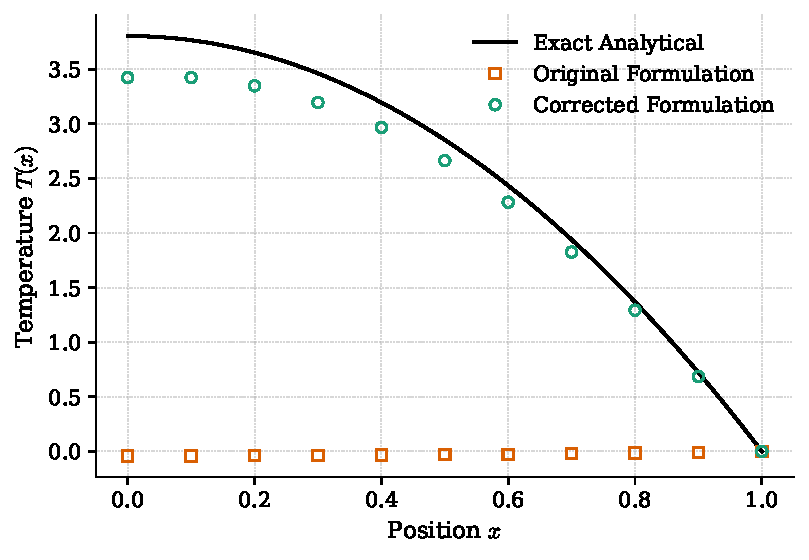
\includegraphics[width=0.85\textwidth]{figures/temperature_comparison.pdf}
    \caption{Comparison between the analytical temperature profile, the solution obtained from the original prescribed formulation, and the corrected finite-difference solution.}
    \label{fig:temperature-comparison}
\end{figure}

To validate the corrected method, an auxiliary convergence experiment was performed using grid sizes $N \in \{11, 21, 41, 81\}$. As shown in \autoref{tab:convergence}, the error monotonically decreases as $h \to 0$.

\begin{table}[ht]
    \centering
    \caption{Empirical convergence of the corrected finite-difference formulation.}
    \label{tab:convergence}
    \begin{tabular}{cccc}
        \toprule
        $N$ & $h$    & $L_\infty$ Error & $L_2$ Error \\
        \midrule
        11  & 0.1000 & 3.8039e-01       & 2.3602e-01  \\
        21  & 0.0500 & 1.9019e-01       & 1.1392e-01  \\
        41  & 0.0250 & 9.5097e-02       & 5.5933e-02  \\
        81  & 0.0125 & 4.7548e-02       & 2.7709e-02  \\
        \bottomrule
    \end{tabular}
\end{table}

The computed convergence rate in the $L_\infty$-norm is approximately $1.00$, and in the $L_2$-norm is approximately $1.03$. This first-order convergence behavior is mathematically expected because a first-order forward difference approximation was employed for the boundary condition at $x=0$, effectively bottlenecking the global accuracy of the second-order interior scheme.

\subsection{Physical Interpretation}

The stated steady-state boundary-value problem describes a one-dimensional bar subject to a constant internal heat source $f > 0$. The zero-flux Neumann boundary condition at $x=0$ models a perfectly insulated edge, while the homogeneous Dirichlet boundary condition at $x=1$ fixes the right edge to a baseline reference temperature of zero. Physically, thermal energy is continuously generated inside the domain and is completely blocked from exiting via the left boundary; therefore, all generated heat must flow rightwards to dissipate. This mechanism produces a temperature profile that is concave downward and reaches its maximum at the insulated boundary. The corrected numerical solution reproduces these qualitative features and approaches the analytical profile as the grid is refined.

By contrast, the original algorithmic formulation uses a discrete operator with the sign of the positive second derivative, together with the nonstandard source scaling described above. At the prescribed grid, this produces a concave-up profile with temperatures below the reference value imposed at $x=1$. This behavior is a consequence of the inconsistency between the generated discrete system and the stated differential equation, not evidence of numerical instability in the linear solve.
